\documentclass[letterpaper]{article}
\usepackage{natbib,alifexi}
\usepackage[T1]{fontenc}
\usepackage{lmodern}
\usepackage[utf8]{inputenc}
\usepackage{abstract}
\usepackage{textcomp}
\usepackage{amsmath}
\usepackage{graphicx}
\usepackage{placeins}

\title{Study of various algorithms for identifying tones in musical audio files, and proposal of an efficient and suited Clojure implementation}
\author{Antoine Passemiers$$ \\
\mbox{}\\
$$Université Libre de Bruxelles \\
apassemi@ulb.ac.be}

\begin{document}
\maketitle

\renewcommand\bibname{Bibliographie}        % Change the bib title
\renewcommand{\refname}{Bibliographie}



\begin{abstract}
The project involves the discussion of different approaches to automated tone detection in audio files,
the prototyping of these methods in Python, a quick reflexion on their consistency with functional programming,
and the implementation of the most appropriate one in Clojure.
State of the art comprises various pitch class profile (PCP) approaches and machine learning algorithms, and this
report aims to implement all of them to be able to discuss them according to their accuracy.

\end{abstract}

\section*{1. Introduction}

The tone of a musical work is characterised by the set of sounds coming from a same diatonic scale.
Unlike scales, where musical notes follow each other in a contiguous manner, tones assemble notes that can be
disjoined or even overlapped. \citep{AD} 
Therefore, our central concern is the analysis of polyphonic melodies, which constitute the overwhelming
majority of the modern musical works.\\

More specifically, we will give consideration to two types of tonality prediction methods :
those based on tone profiles, and those based on machine learning algorithms. Most of the latter base their design on the
markovian property

[[En particulier, nous allons nous pencher sur deux catégories d\textquotesingle algorithmes :
ceux basés sur des modèles cognitifs, et ceux incluant des notions d\textquotesingle 
apprentissage automatique. Les premiers tentent d\textquotesingle intégrer au mieux les connaissances
de la théorie musicale et reposent sur la façon dont les personnes reconnaissent les différentes tonalités,
alors que les seconds utilisent l\textquotesingle inférence statistique pour déterminer celles-ci.\\]]

[[L\textquotesingle approche cognitive utilisée pour la détection de la tonalité repose en partie
sur la solution proposée par Ibrahim Sha\textquotesingle ath lors 
de la conception du logiciel KeyFinder \citep{IS}. La précision de la détection est évaluée 
à l\textquotesingle aide d\textquotesingle une base 
de données, constituée de 250 fichiers musicaux au format wav, dont les tonalités sont connues
et inscrites dans un fichier csv. Ces fichiers font partie de ceux utilisés par 
Ibrahim Sha\textquotesingle ath dans le cadre de sa recherche.\\]]

Pour ce qui est de la partie apprentissage automatique, les méthodes présentées seront principalement
en lien avec les modèles de Markov cachés. Leur évaluation se fera en divisant la base de données en
un jeu de données d\textquotesingle apprentissage et un jeu de données de validation (respectivement
60 \% et 40 \% du jeu de données d\textquotesingle origine). Ce mini-mémoire se voulant concis et 
centré sur les objectifs décrits, le lecteur est supposé déjà disposer de connaissances suffisantes en 
apprentissage automatique, en théorie musicale et en traitement logiciel de signaux.

TODO : \citep{SP} \citep{AT} -> Partie 2.1.1.

\section*{2. Theoretical considerations}

\subsection*{2.1. Preprocessing}

The audio signal is first extracted from the wav file, and then the average of its channels is calculated
if the file has been written in stereo. It is not required to take the pan into account given that mixing
channels or analysing the channels separately makes no difference in the spectral domain. Also, there is
no indispensable need to consider the whole frequential spectrum given that notes are mainly characterised 
by their fundamental frequency
and that the harmonics of the highest notes are not relevant for estimating chroma vectors.
The sampling rate is de facto resampled at a tenth of the standard sampling frequency (4410 Hz).
Although this drastic downsampling is likely to create aliasing effects (which can be simply avoided by 
applying a low-pass filter), no loss of accuracy has been pointed out during the evaluation phase.

\subsection*{2.2. Spectral estimation}

Il existe deux catégories de techniques d\textquotesingle estimation de densité spectrale : les méthodes paramétriques et les méthodes non-paramétriques.


\subsubsection*{2.2.1. Constant-Q Transform (CQT)}

Avant de procéder à l\textquotesingle estimation de la CQT, une fenêtre de Blackman est appliquée sur les données observées afin d\textquotesingle
 éviter les distortions spectrales dues à l\textquotesingle étroitesse de la fenêtre (et au principe d\textquotesingle incertitude d\textquotesingle Heisenberg).
Le spectre est alors approximé à l\textquotesingle aide de la transformée de Fourier rapide (FFT). L\textquotesingle intuition derrière la Constant-Q 
Transform (CQT)
est de penser que les coefficients de la FFT dont les fréquences ne correspondent pas à des notes de musique prennent plus de poids que les autres
coefficients. Ceci doit être réajusté en appliquant des fenêtres spectrales centrées sur les notes de musiques. Pour chaque fenêtre, les coefficients résultants de cette opération sont alors sommés pour ne former qu\textquotesingle un seul coefficient spectral. L\textquotesingle ensemble des coefficients globaux
constitue alors la CQT.


\subsubsection*{2.2.2. Pisarenko Harmonic Decomposition (PHD)}



\citep{MA}

\subsubsection*{2.2.3. Least-squares spectral estimation}

It is also possible to estimate the spectrum using dedicated regression techniques. We will give focus on the most popular of them :
the Van\'{\i}\v{c}ek method and the Lomb-Scargle method. A spectrum approximated by one of the latter is called a periodogram.
The incentives for the Van\'{\i}\v{c}ek method are to be able to handle missing data samples, since it has been developped in the fields of
geology and astrophysics, where data are not received at regular intervals. Furthermore, unlike the Fast Fourier Transform which has a
variable spectral resolution (depending on the size of the observation window), the least-squares methods output periodograms of a size
that is equal to the number of frequencies of interest. The more frequencies we will consider, the longer the execution time will be.
It is a great concern as well that both Van\'{\i}\v{c}ek and Lomb-Scargle methods make the assumption that signals consist of a
linear combination of sine-waves and white noise (where the sine-wave frequencies are known), and the assumption that the signal has an 
offset of zero.

\begin{align}
\hat{\theta}_{k} = (A_{k}^{T} A_{k})^{-1} A_{k}^{T} y
\end{align}

According to the Van\'{\i}\v{c}ek method, the coefficients of the linear combination are stored in a vector $\theta_{k}$, in such a way that
the signal equals $y \approx A\theta_{k}$. Each row of the matrix A contains the data samples of the sine-wave of a particular frequency of interest.
Finally, the coefficients are given by the equation 1. \citep{PS}\\

[[ Le défaut de la méthode est de ne pas considérer les phases des fréquences concernées. En effet chaque sinusoïde contenue dans la matrice A
est supposée posséder une phase nulle. La méthode de Lomb-Scargle permet de résoudre ce problème en pré-calculant les phases des sinusoïdes
utilisées et en tenant compte au mieux de celles-ci lors du calcul du spectre. Le déphasage $\tau$ correspondant à la fréquence $f$ est donné par
l\textquotesingle équation 2. \citep{LS} ]]

\begin{align}
\tan 2\pi f \tau = \frac{\sum\limits_{j=1} \sin 2\pi f t_{j}}{\sum\limits_{j=1} \cos 2\pi f t_{j}}
\end{align}

[[ Tout comme dans la méthode de Vanícek, la régression consiste en la recherche de coefficients qui expliquent au mieux le signal sous la forme d\textquotesingle
une pondération de sinusoïdes. Le coefficient associé à la fréquence $f$ est donné par l\textquotesingle équation 3 : ]]

\begin{align}
\Delta R(f) = \frac{(YC)^{2}}{CC} 
+ \frac{(YS)^{2}}{SS}
\end{align}

CC and SS values are computed only once (when the namespace is loaded), since the frequencies of interest don’t change from a wav file to another.

\begin{align}
CC = \sum\limits_{j=1} \cos^{2} 2\pi f (t_{j} - \tau)
\end{align}

\begin{align}
SS = \sum\limits_{j=1} \sin^{2} 2\pi f (t_{j} - \tau)
\end{align}

[[Les valeurs YC et YS cherchent à mesurer respectivement les niveau d\textquotesingle orthogonalité du signal $y$ avec une sinusoïde déphasée de $\pi / 2$ et avec une sinusoïde de phase nulle. Ces sinusoïdes peuvent également être pré-calculées. Les formules permettant de calculer YC et YS sont : ]]

\begin{align}
YC = \sum\limits_{j=1} y_{j}\cos 2\pi f (t_{j} - \tau)
\end{align}

\begin{align}
YS = \sum\limits_{j=1} y_{j}\sin 2\pi f (t_{j} - \tau)
\end{align}

Ainsi, les seules opérations restantes lors de l\textquotesingle exécution de l\textquotesingle algorithme sont les produits scalaires entre les
sinusoïdes et le signal délimité par la fenêtre glissante, ce qui réduit drastiquement la quantité de calculs requis pour l\textquotesingle estimation du spectre.

\subsubsection*{2.2.4. Other approaches}

TODO : Cepstral coefficients, ...

\subsection*{2.3. Key identification}

Une fois le spectre estimé, celui-ci est compacté dans un vecteur chromatique composé de douze coefficients. Dans le cadre de l\textquotesingle évaluation de l\textquotesingle algorithme, il a été trouvé que 6 octaves suffisent à approximer le spectre : l\textquotesingle ajout d\textquotesingle une septième octave n\textquotesingle améliore pas la précision des prédictions. De fait, le spectre dont la résolution est de 72 coefficients (12 x 6 octaves) est redimensionné en une matrice $M_{i, j}$ de dimensions (6 x 12). Enfin, le vecteur chromatique $C_{i}$ est obtenu en formalisant la méthode élaborée par Sha\textquotesingle ath :

\begin{align}
C_{i} = (1 - p) * \max_{j} M_{i, j} + p * \sum_{j} M_{i, j}
\end{align}

où p est un hyper-paramètre déterminé durant l\textquotesingle évaluation/validation de l\textquotesingle algorithme. La dernière étape consiste alors à identifier localement la tonalité sur base unique de ce vecteur chromatique. Différentes méthodes ont été discutées, la première se base sur la méthode de
Sh\textquotesingle ath alors que les suivantes reposent sur des algorithmes d\textquotesingle apprentissage automatique.

\subsubsection*{2.3.1. Modèle cognitif}

Cette solution repose sur les expériences menées par Carol L. Krumhansl et Lola L. Cuddy sur la perception des tonalités chez l\textquotesingle Homme.
Des gammes incomplètes ont été jouées, suivies de notes additionnelles que les sujets devaient évaluer sur leur capacité à compéter ces gammes. 
Les scores ont été moyennés pour donner les deux graphiques suivants :

\FloatBarrier

\begin{figure}[h!]
\begin{center}
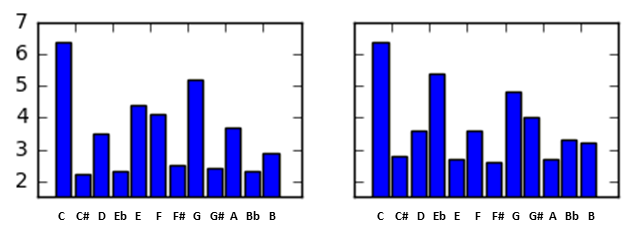
\includegraphics[width=3.1in,angle=0]{imgs/Krumhansl.png}
\caption{Profils de tonalités dérivés de l\textquotesingle expérience de Krumhansl, et représentant respectivement la gamme do majeur
et la gamme do mineur.}
\label{fig1}
\end{center}
\end{figure}

Bien que ces deux profils de tonalités fournissent des résultats satisfaisants lorsque le spectre est estimé à l\textquotesingle aide de la CQT, il ne sont pas adaptés lorsque la méthode de Lomb-Scargle est utilisée, car il a été observé que les coefficients renvoyés par cette dernières sont globalement plus equidistribués. Cette distribution doit se refléter dans les profils de tonalité, c\textquotesingle est pourquoi l\textquotesingle algorithme a été évalué plusieurs fois jusqu\textquotesingle à obtenir les profils fournissant les meilleurs résultats, et donnés ci-dessous :

\begin{figure}[h!]
\begin{center}
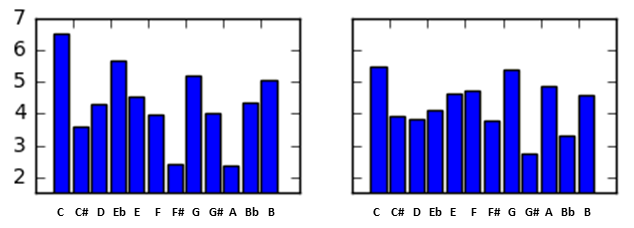
\includegraphics[width=3.1in,angle=0]{imgs/Custom.png}
\caption{Meilleurs profils de tonalités, déterminés empiriquement}
\label{fig1}
\end{center}
\end{figure}

\FloatBarrier

\subsubsection*{2.3.2. Hidden Markov Models (HMM)}

Hidden Markov Models are discrete state machines that represent multivariate series by their distributions and by
the transition probailities between their states. Their states are called “hidden” because they are not observed directly,
but can be inferred from the observation sequence using a parameter estimation method (such as the expectation-maximization algorithm
or the Viterbi algorithm). Each hidden state distinguishes itself by its emission probabilities (or emission probability density function).
Unlike more popular machine learning models such as neural networks or support vector machines (SVM), Hidden Markov Models are capable of
processing input sequences of variable length. This characteristic is substantial given that music tracks are of variable length by nature.\\

The old-fashioned way to classify keys using HMMs consists of training a HMM for each distinct music key, and to predict the most probable 
key of an unlabelled music track by looking for the HMM that maximizes the track\textquotesingle s log-likelihood.

TODO : \citep{JP} \citep{DR}

\subsubsection{2.2.3. Feedforward neural networks}

Neural networks have already delivered good results for classifying chords inside a same piece of music.

\subsubsection*{2.2.4. Input-Output Hidden Markov Models (IO-HMM)}

The main deficiency of the standard HMM is that it has no discriminative capabilities : if one of the keys appears to be more frequent in the database or
if it seems to be easily explained by the HMM, the latter will present high risks of predicting the same key every time, regardless of the
input sequence. On the other hand, feedforward neural networks have the defect that they are not suited for temporal data, since they must 
process features of fixed size. [[ TODO : recurrent networks ]]

The Input-Output Hidden Markov Model is well suited for our task because it is affected by none of these deficiencies.

TODO : \citep{YB}

\subsection*{2.4. Methodology}

\subsubsection{2.4.1. Datasets}

The database consists of 415 music tracks recorded in wav format, 44100 Hz stereo. Each wav file has an associated key. All keys have been determined
by experts and have been made available by Ibrahim Shat\textquotesingle ath as part of its work. For evaluating algorithms based on tone profiles,
all the tracks have been used to tune the parameters to their best value. The latter consist of : the major and minor tone profile coefficients,
the size of the sliding window, and the range of the spectrum frequency bins. For evaluating machine learning techniques,
the dataset is split into a training set of 138 music tracks and a validation set of 277 tracks.

\subsubsection{2.4.2. Evaluation}

In the framework of this study, we consider only the twelve heptatonic major scales and the twelve heptatonic minor scales.
Two different metrics are used to evaluate the accuracy of the algorithms :
the raw accuracy (the ratio between the number of correct predictions to the number of analyzed files) and the MIREX index.
The MIREX metric is a weighted sum of the number of correct predictions (C), the number of predictions that are out by a fifth (F), 
out by a fourth (U), the number of predicted scales that are parallel to the correct ones (P), and the number of predicted scales
that are relative to the correct ones (R). The index is then given by : \\

$ MIREX = (C + \frac{1}{2}.F + \frac{1}{2}.U + \frac{3}{10}.R + \frac{1}{5}.F) / TOTAL $

\subsubsection*{2.5. Results}

\FloatBarrier

\begin{table}[h!]
\center{
\begin{tabular}{|c|c|c|}\hline
Méthode & Précision & MIREX \\ \hline\hline
CQT + profiles & 30,7\%  & - \\
Lomb-Scargle + profiles & 36,6\% & 49,4\% \\
CQT + HMM & -- & -- \\
FFT + IO-HMM & -- & -- \\
CQT + IO-HMM & -- & -- \\ 
Lomb-Scargle + IO-HMM & -- & -- \\ 
\hline
\end{tabular}
}
\vskip 0.25cm
\caption{Accuracy assessment, according to the raw accuracy and the MIREX index}
\end{table}

\FloatBarrier

\section{3. Clojure implementation}

Clojure is a dynamic and functional programming language based on the Java Virtual Machine, suited for quickly designing multithreaded programs,
and featuring a full range of persistent data structures.

\begin{figure}[h!]
\begin{center}
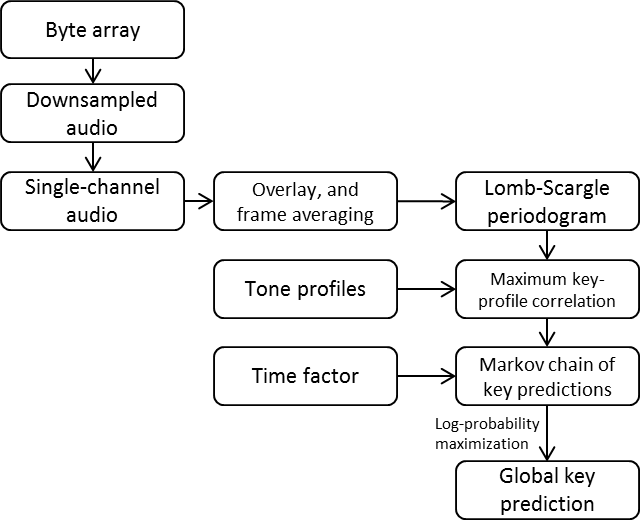
\includegraphics[width=3.1in,angle=0]{imgs/flowChart.png}
\caption{Flowchart of the solution design}
\label{fig3}
\end{center}
\end{figure}

TODO : \citep{SK}


\footnotesize
\bibliographystyle{apalike}
\bibliography{thesis}


\end{document}